\begin{frame}
\frametitle{Model: Overview}
\begin{center}
input layer output layer magic processing output
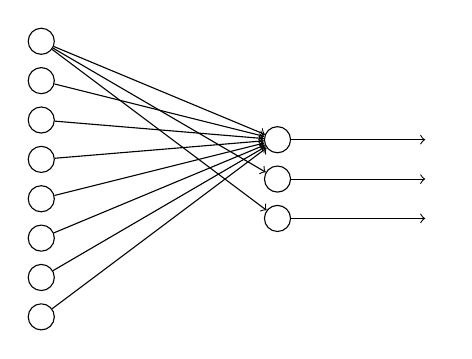
\begin{tikzpicture}[->]

	% draw input layer
	\foreach \s in {0,...,7}
	{
		\node[draw, circle] (i_\s) at (0,-\s * 0.5) {};
	}
	
	% draw output layer	
	\foreach \s in {0,...,2}
	{
		\node[draw, circle] (o_\s) at (3,-1.25 -\s * 0.5) {};
		\node (m_\s) at (5,-1.25 -\s * 0.5) {};
		\path (o_\s) edge node {} (m_\s);
	}
	
	% draw edges
	\foreach \s in {0,...,7}
	{
			\path (i_\s) edge node {} (o_0);
	}
	\path (i_0) edge node {} (o_1);
	\path (i_0) edge node {} (o_2);

\end{tikzpicture}
\end{center}
\end{frame}


\begin{frame}
\frametitle{Model: Input Layer}
\begin{tikzpicture}[overlay,remember picture]
\node[anchor=north west] at ($(current page.north west)+(0,-1)$) {
  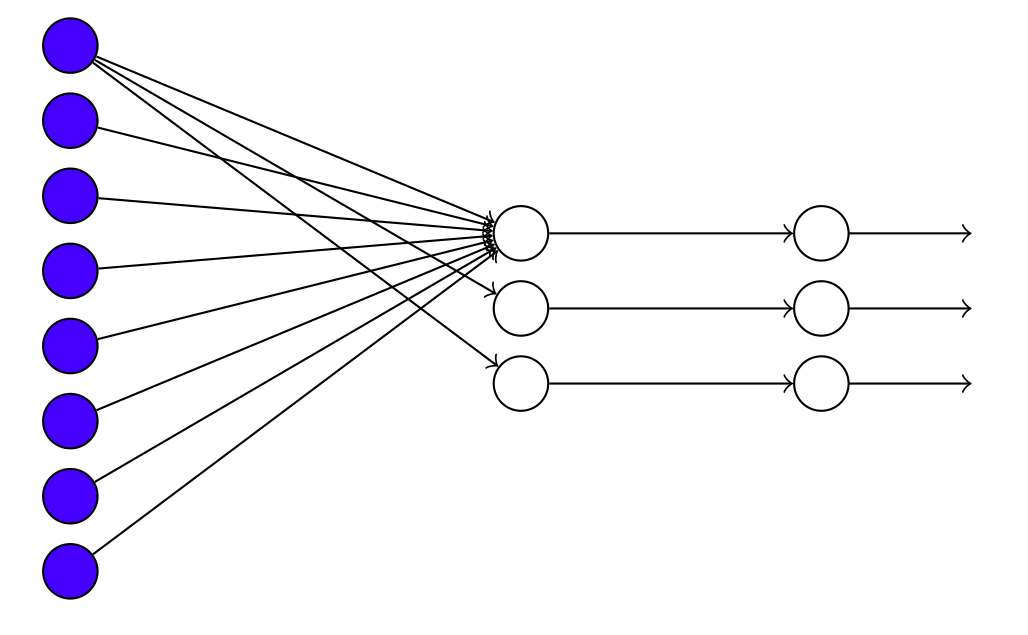
\includegraphics[scale=.1]{pics/model_input}
};
\node[anchor=north east] at ($(current page.north east)+(-2,-1.5)$) {
  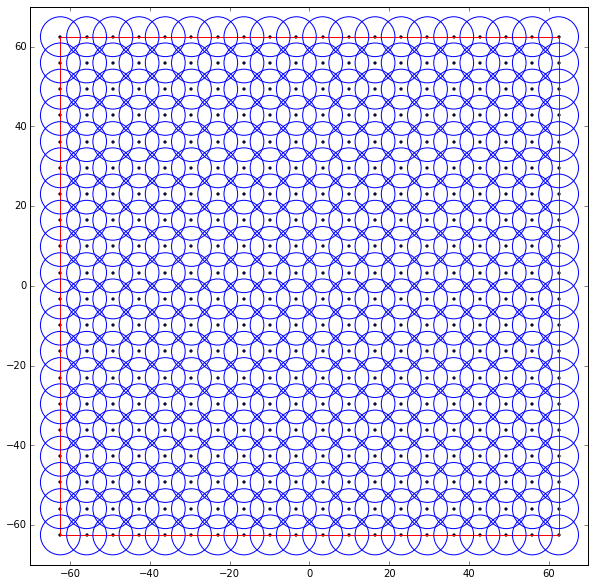
\includegraphics[scale=.2]{pics/place_cell_locations}
};
\node[anchor=south west] at ($(current page.south west)+(1,1)$) {
  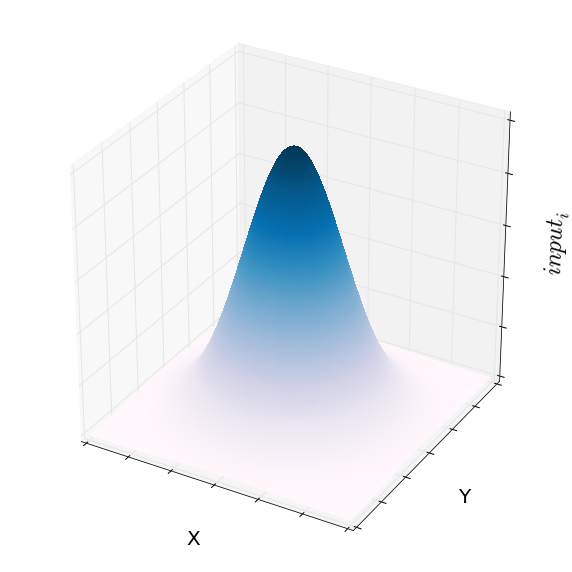
\includegraphics[scale=.2]{pics/gauss}
};
\node[anchor=south east] at ($(current page.south east)+(-1.5,2)$) {
  \footnotesize{$input_i = \exp(-\frac{||rat\_pos - center_i||^2}{50})$}
};
\end{tikzpicture}
\end{frame}


\begin{frame}
\frametitle{Model: Input Layer}
\begin{tikzpicture}[overlay,remember picture]
\node[anchor=north west] at ($(current page.north west)+(0,-1)$) {
  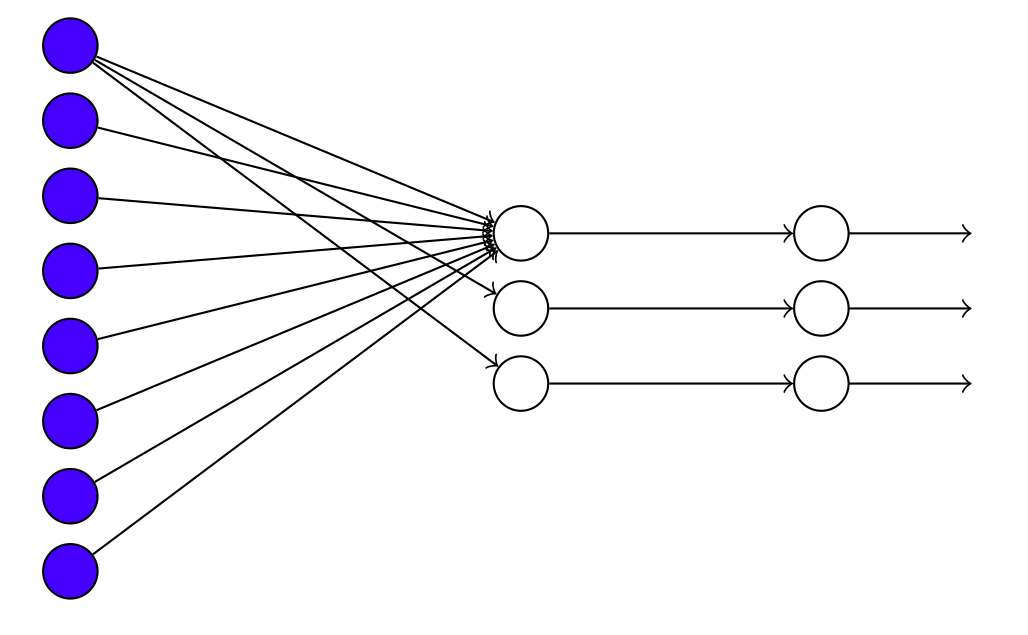
\includegraphics[scale=.1]{pics/model_input}
};
\node[anchor=north east] at ($(current page.north east)+(-1.5,-1.5)$) {
  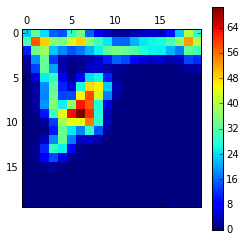
\includegraphics[scale=.55]{pics/activity_demo}
};
\node[anchor=south west] at ($(current page.south west)+(1,1)$) {
  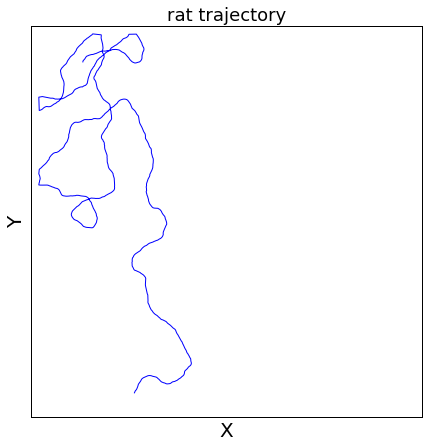
\includegraphics[scale=.27]{pics/mouse_demo}
};
\end{tikzpicture}
\end{frame}


\begin{frame}
\frametitle{Model: Output Layer}
\begin{multicols}{2}
\begin{center}
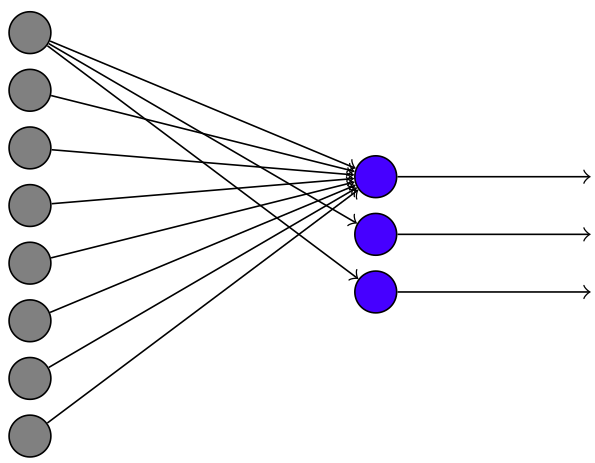
\includegraphics[scale=.1]{pics/model_output}
\end{center}
\columnbreak
\begin{center}
$h_j = \sum_i w_{ij} \cdot input_i$
\end{center}
\end{multicols}
\end{frame}

\begin{frame}
\frametitle{Model: Output Layer}
\begin{multicols}{2}
\begin{center}
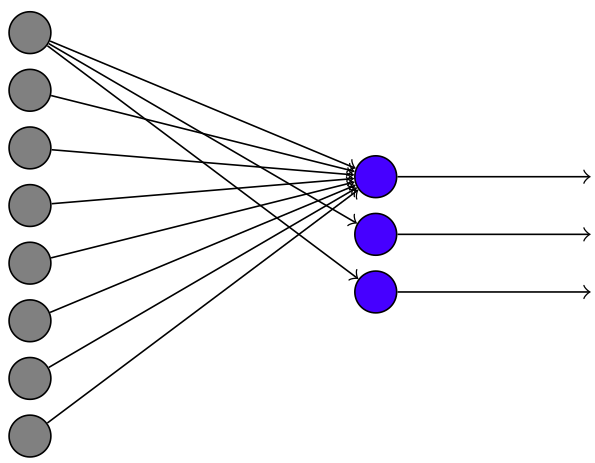
\includegraphics[scale=.1]{pics/model_output}
\end{center}
\columnbreak
\begin{center}
$h_j(t) = \sum_i w_{ij} \cdot input_i(t)$\\
\vskip 6mm
$\rightarrow$ adaptation dynamics:\\
\vskip 3mm
$\tau^+\frac{d}{dt}r^+_j=h_j(t)-r^+_j(t)-r^-_j(t)$\\
\vskip 3mm
$\tau^-\frac{d}{dt}r^-_j(t)=r^-_j(t)$
\vskip 5mm
\end{center}
\end{multicols}
\end{frame}

\begin{frame}
\frametitle{Model: Output Layer}
\begin{multicols}{2}
\begin{center}
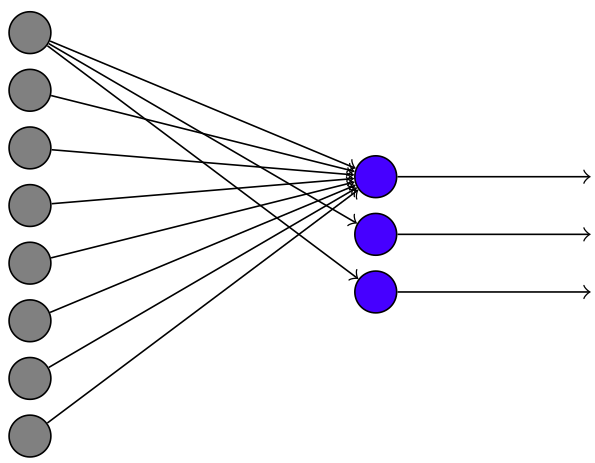
\includegraphics[scale=.1]{pics/model_output}
\vskip 3mm
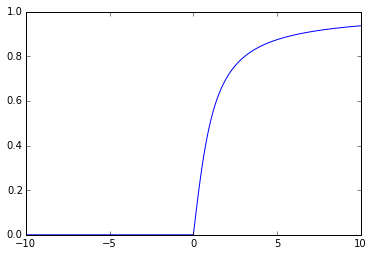
\includegraphics[scale=.3]{pics/output_function}
\end{center}
\columnbreak
\begin{center}
$h_j(t) = \sum_i w_{ij} \cdot input_i(t)$\\
\vskip 6mm
$\rightarrow$ adaptation dynamics:\\
\vskip 3mm
$\tau^+\frac{d}{dt}r^+_j=h_j(t)-r^+_j(t)-r^-_j(t)$\\
\vskip 3mm
$\tau^-\frac{d}{dt}r^-_j(t)=r^-_j(t)$\\
\vskip 3mm
$\rightarrow$ output:\\
\vskip 3mm
$output_j(t)=\frac{2}{\pi} \arctan (g \cdot (r^+_j(t)-\mu)) \cdot \theta(r_j^+(t)-\mu)$\\
\vskip 3mm
$g$ - gain, $\mu$ - threshold
\end{center}
\end{multicols}
\end{frame}

\begin{frame}
\frametitle{Model: Weight Updates}
\begin{multicols}{2}
\begin{center}
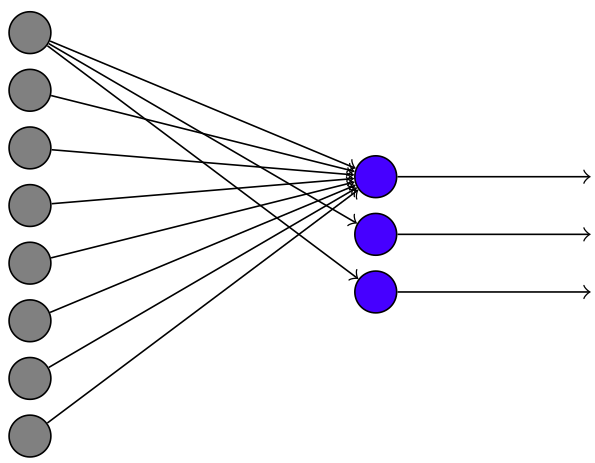
\includegraphics[scale=.1]{pics/model_output}
\end{center}
\columnbreak
\begin{center}
$h_j = \sum_i w_{ij} \cdot input_i$
\vskip 5mm
$\rightarrow$ How to determine\\ \hskip 4mm the weights $w_{ij}$?\\
$\rightarrow$ Hebbian learning dynamics\\
\vskip 4mm
$w_{ij}(t+\Delta)=w_{ij}(t)+$\\
$ \epsilon (input_i(t)\cdot output_j - \sum_s input_i (s) \cdot \sum_s output_j(s))$
\end{center}
\end{multicols}
\end{frame}
